\documentclass{standalone}
\usepackage{picture,color}
\usepackage{graphicx}
\graphicspath{{./Fig_INTRO_subfigs/}}
\setlength{\unitlength}{1in}
\usepackage{helvet}
\renewcommand{\familydefault}{\sfdefault}
\begin{document}
\begin{picture}(6.5, 4.95)(0,-5.66)
\put(0.25, -2.42){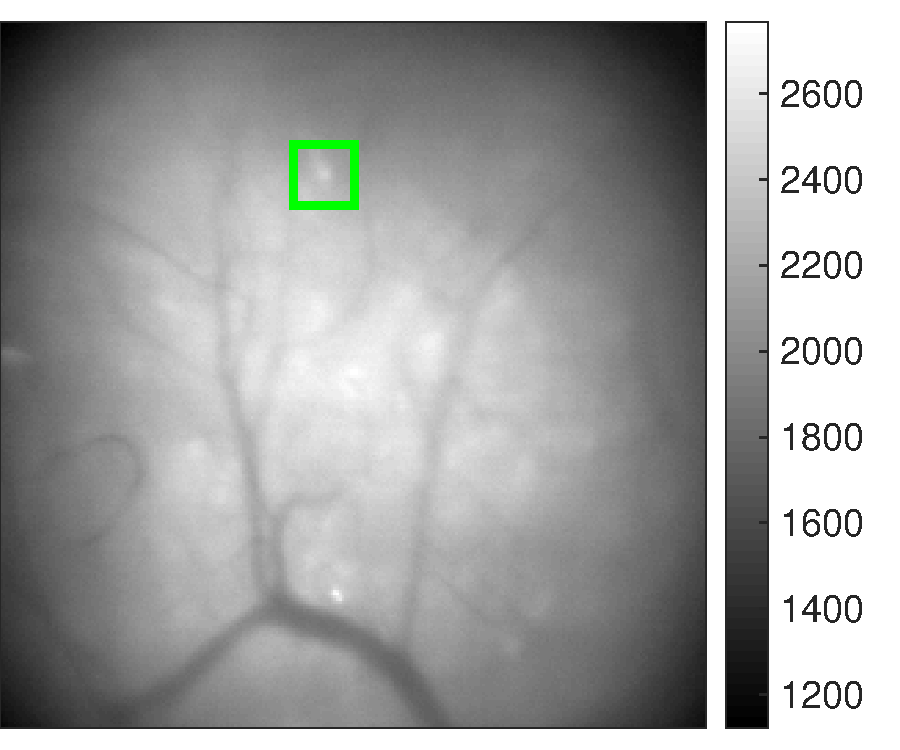
\includegraphics[height=1.5in]{Fig_INTRO_subfigs/example_frame.pdf}}
\put(0.05, -0.95){\large\textbf{A}}
\put(0.65, -0.9){Raw data}

\put(2.45, -2.45){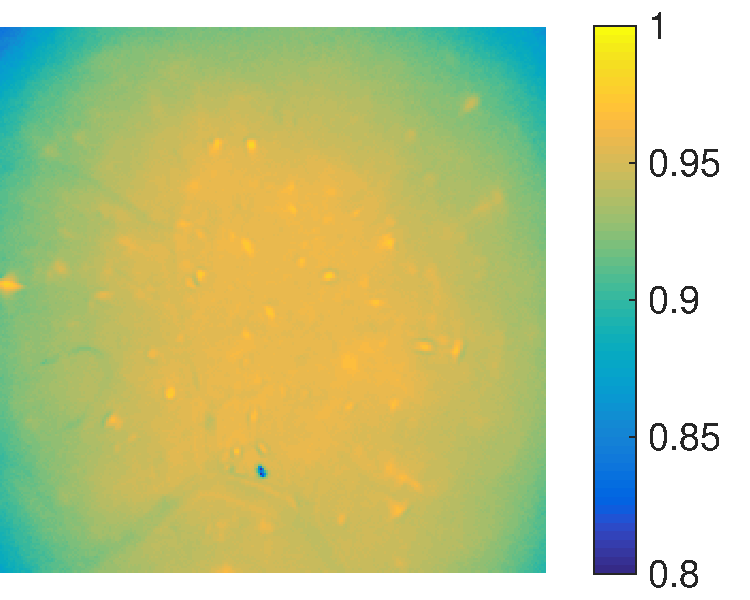
\includegraphics[height=1.56in]{Fig_INTRO_subfigs/correlation_image.pdf}}
\put(2.25, -0.95){\large\textbf{B}}
\put(2.6, -0.9){Correlation image}

% \put(5.5, -1.15){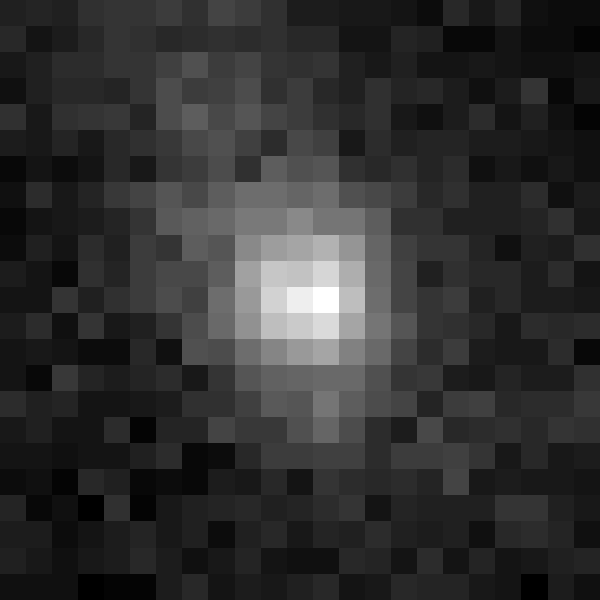
\includegraphics[height=0.69in]{Fig_INTRO_subfigs/example_frame_box_no_baseline.pdf}}
\put(4.8, -2.38){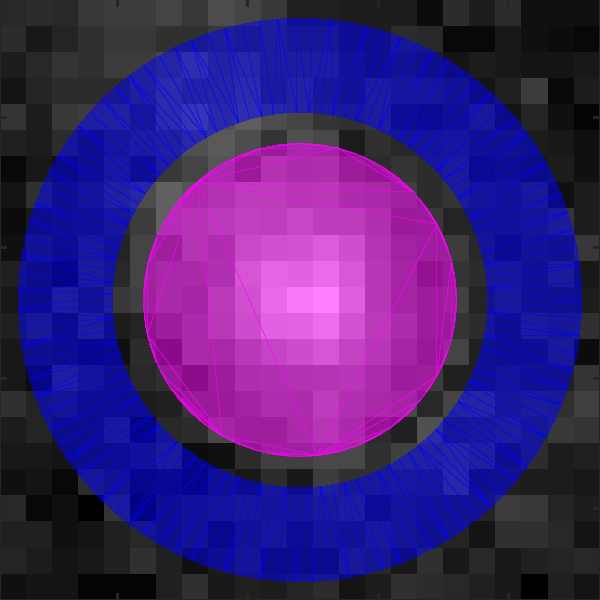
\includegraphics[height=1.42in]{Fig_INTRO_subfigs/example_box_roi.pdf}}
\put(5.2,-0.9){Raw-mean}
\put(4.55, -0.95){\large\textbf{C}}

\put(0.2, -4.1){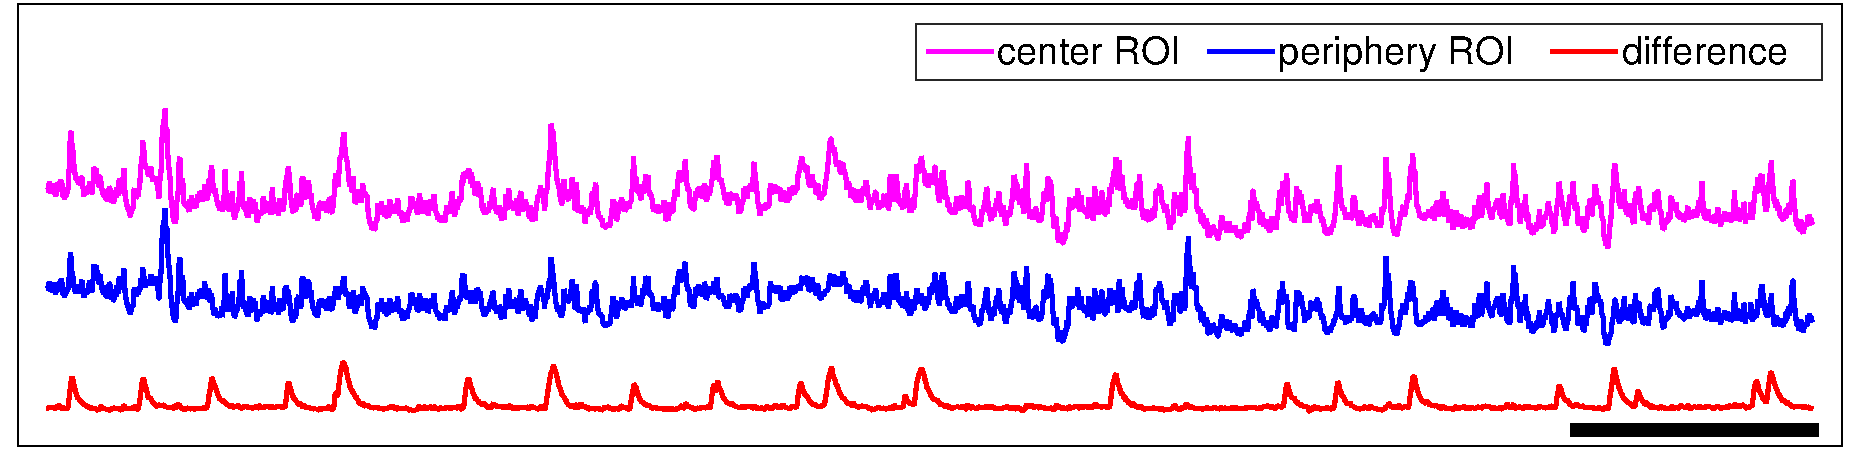
\includegraphics[height=1.51in]{Fig_INTRO_subfigs/example_box_trace.pdf}}
\put(0.05, -2.6){\large\textbf{D}}
% \put(2.86,-2.55){Fluorescence traces}

\put(0.1, -5.65){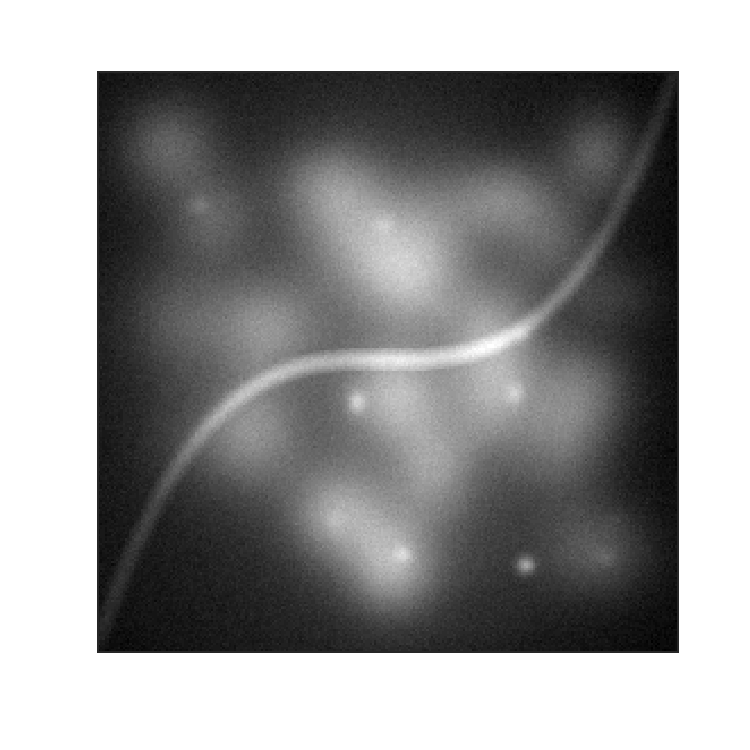
\includegraphics[width=1.35in]{./Fig_BG_subfigs/example_frame.pdf}}
\put(0.05, -4.4){\large\textbf{E}}
\put(0.43, -4.35){{Fluo. signals}}

\put(1.45, -5.65){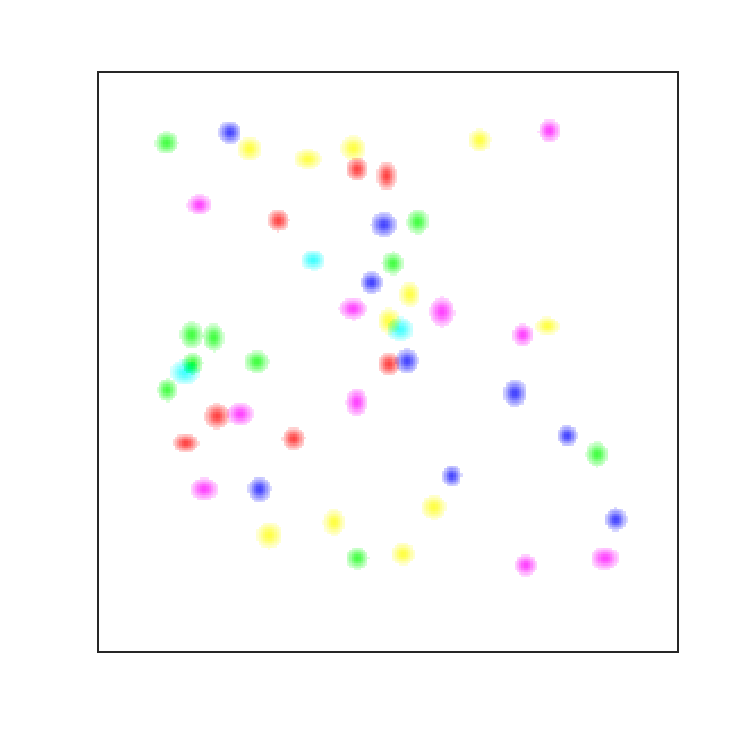
\includegraphics[width=1.35in]{./Fig_BG_subfigs/example_neurons.pdf}}
% \put(1.3, -4.52){\large\textbf{F}}
\put(1.9, -4.35){{Neurons}}
\put(1.4, -5.0){\Large$=$}

\put(2.7, -5.65){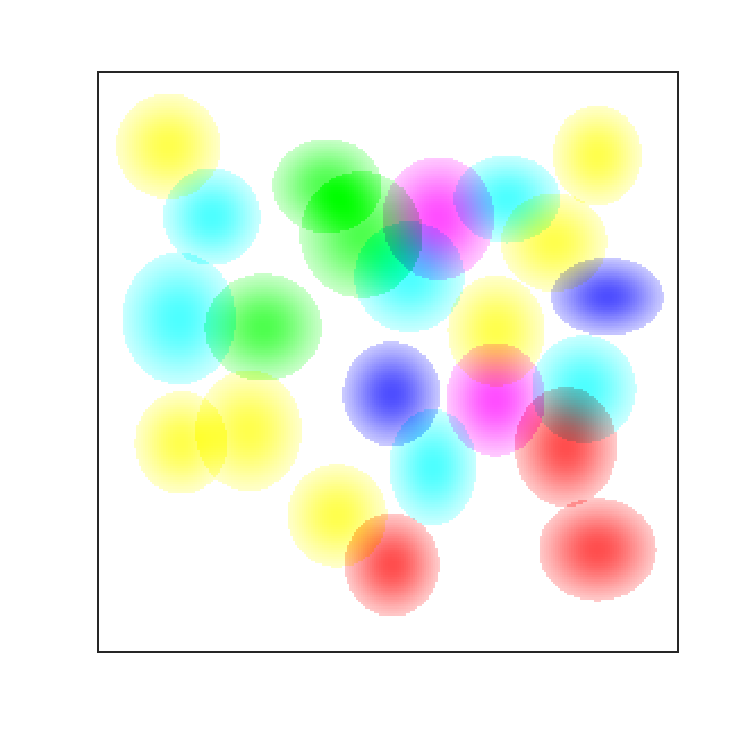
\includegraphics[width=1.35in]{./Fig_BG_subfigs/example_localBG.pdf}}
% \put(2.6, -4.52){\large\textbf{G}}
\put(3.1, -4.35){{Local BG}}
\put(2.7, -5.0){\Large$+$}

\put(3.95, -5.65){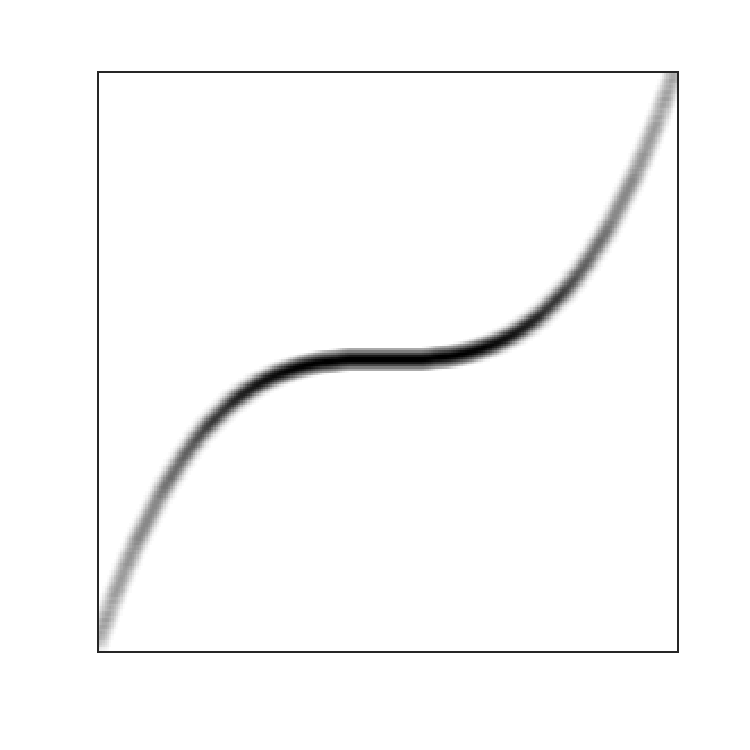
\includegraphics[width=1.35in]{./Fig_BG_subfigs/example_bloodVessel.pdf}}
% \put(3.9, -4.52){\large\textbf{H}}
\put(4.25, -4.35){{Blood vessel}}
\put(3.95, -5.0){\Large$+$}

\put(5.2, -5.65){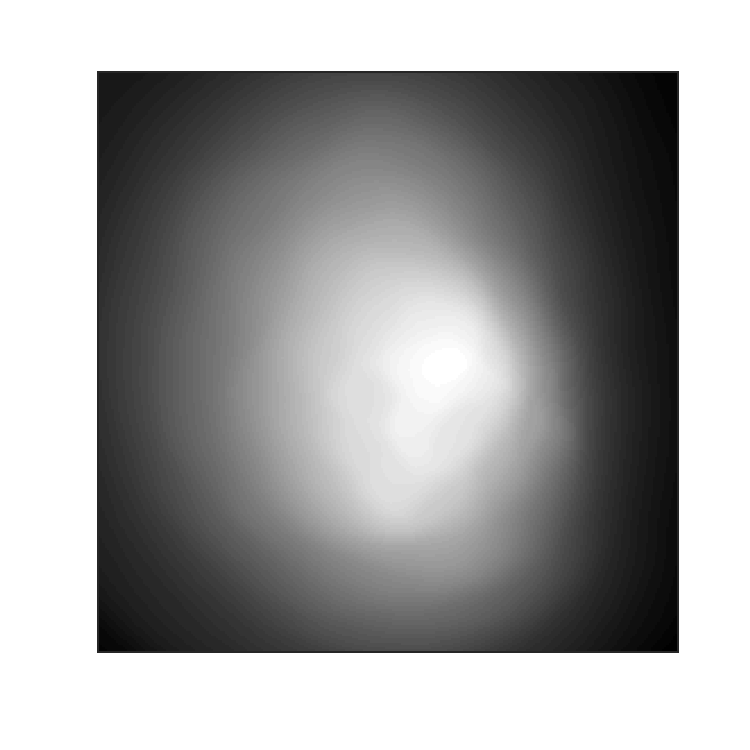
\includegraphics[width=1.35in]{./Fig_BG_subfigs/example_global.pdf}}
% \put(5.2, -4.52){\large\textbf{I}}
\put(5.55, -4.35){{Global BG}}
\put(5.2, -5.0){\Large$+$}

\end{picture}
\end{document}
